\section{Phạm vi đánh giá và cách diễn giải chỉ số}
\label{sec:pham-vi-ket-qua}

Chương này trình bày kết quả đánh giá các mô hình phân loại nhị phân trên UNSW-NB15, với Normal = 0 và Attack = 1. Official TRAIN có 175\,341 dòng; official TEST có 82\,332 dòng, gồm 37\,000 Normal và 45\,332 Attack. Ba pipeline cuối là Random Forest 42 đặc trưng (RF-42), Stacking 42 đặc trưng (Stacking-42) và Random Forest 17 đặc trưng (RF-17); cả ba dùng ngưỡng phân loại 0,5. Các biến \texttt{id}, \texttt{label} và \texttt{attack\_cat} không được dùng làm predictor. Trường \texttt{attack\_cat} chỉ hỗ trợ phân tích hậu nghiệm các mẫu Attack bị bỏ sót, không đại diện cho kết quả phân loại đa lớp.

Với Attack là lớp dương, FPR là tỷ lệ Normal bị gán nhầm thành Attack, còn FNR là tỷ lệ Attack bị bỏ sót:
\begin{equation}
  \mathrm{FPR}=\frac{\mathrm{FP}}{\mathrm{TN}+\mathrm{FP}},
  \qquad
  \mathrm{FNR}=\frac{\mathrm{FN}}{\mathrm{TP}+\mathrm{FN}},
  \qquad
  \mathrm{Detection\ Rate}=1-\mathrm{FNR}.
\end{equation}
Macro-F1 cho trọng số bằng nhau giữa hai lớp; MCC tổng hợp sự phù hợp giữa dự đoán và nhãn qua confusion matrix. Vì vậy, hai chỉ số này được đọc cùng số FP/FN và không dùng Accuracy đơn lẻ để xếp hạng pipeline.

\section{Kết quả trên official holdout}
\label{sec:ket-qua-official}

Bảng~\ref{tab:ket-qua-official} cho thấy cả ba pipeline phát hiện phần lớn mẫu Attack nhưng vẫn gán nhầm hơn một phần tư số mẫu Normal. Chênh lệch giữa RF-42 và Stacking-42 nhỏ theo Macro-F1 và MCC, trong khi hai loại lỗi thay đổi theo hướng đối nghịch: Stacking giảm FP 142 mẫu, từ 10\,003 xuống 9\,861, nhưng tăng FN 118 mẫu, từ 734 lên 852. Khi chưa có hàm chi phí vận hành để quy đổi cảnh báo giả và bỏ sót thành cùng một thang đo, kết quả này không xác định được cấu hình phù hợp hơn cho mọi bối cảnh sử dụng.

\begin{table}[htbp]
\centering
\small
\renewcommand{\arraystretch}{1.3}
\setlength{\tabcolsep}{6pt}
\caption{Hiệu năng nhị phân trên official TEST (82\,332 mẫu; ngưỡng 0,5).}
\label{tab:ket-qua-official}
\begin{tabularx}{\linewidth}{>{\raggedright\arraybackslash}X S[table-format=1.6] S[table-format=1.6] S[table-format=2.4] S[table-format=1.4] S[table-format=5.0] S[table-format=4.0]}
\toprule
Pipeline & {Macro-F1} & {MCC} & {FPR (\%)} & {FNR (\%)} & {FP} & {FN}\\
\midrule
RF-42 & 0.863343 & 0.750910 & 27.0351 & 1.6192 & 10003 & 734\\
Stacking-42 & 0.863840 & 0.750497 & 26.6514 & 1.8795 & 9861 & 852\\
RF-17 & 0.860673 & 0.746881 & 27.6324 & 1.5618 & 10224 & 708\\
\bottomrule
\end{tabularx}
\end{table}

So với RF-42, RF-17 có Macro-F1 thấp hơn 0.002670, ít hơn 26 FN nhưng nhiều hơn 221 FP. Thời gian huấn luyện và kích thước ước lượng nhỏ hơn đáng kể trong lần chạy lịch sử (Bảng~\ref{tab:chi-phi}), song RF-17 cũng khác RF-42 về số cây và kích thước lá. Do đó, chênh lệch này là đánh đổi giữa hai pipeline, không phải hiệu ứng riêng của việc giảm số đặc trưng.

\begin{figure}[htbp]
\centering
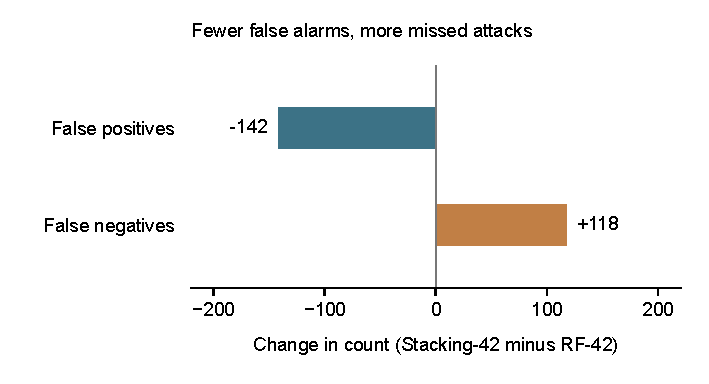
\includegraphics[width=0.82\textwidth]{../results/figures/p16_r05_error_tradeoff/error_tradeoff.pdf}
\caption{Chênh lệch số FP và FN của Stacking-42 so với RF-42 trên cùng official TEST.}
\label{fig:delta-fp-fn}
\end{figure}

\section{Độ bất định của chênh lệch và kiểm định cặp}
\label{sec:bat-dinh}

Bảng~\ref{tab:chenh-lech-ci} trình bày hiệu số Stacking-42 trừ RF-42 cùng khoảng tin cậy paired bootstrap 95\%. CI của Macro-F1 và MCC chứa 0; do đó, dữ liệu chưa cho thấy bằng chứng đủ rõ về ưu thế của Stacking trên hai chỉ số tổng hợp, nhưng cũng không thiết lập tương đương thống kê. McNemar exact sau hiệu chỉnh Holm cho ba cặp mô hình trong view đánh giá tương ứng cho $p_{\mathrm{Holm}}=0.468377$ đối với tính đúng tổng thể. Phép kiểm định này không kiểm định trực tiếp hiệu số Macro-F1.

\begin{table}[htbp]
\centering
\small
\renewcommand{\arraystretch}{1.3}
\setlength{\tabcolsep}{10pt}
\caption{Hiệu số Stacking-42 trừ RF-42 và CI 95\% paired bootstrap trên official TEST; hiệu số ở thang 0--1.}
\label{tab:chenh-lech-ci}
\begin{tabularx}{\linewidth}{X S[table-format=+1.6] S[table-format=+1.6] S[table-format=+1.6]}
\toprule
Chỉ số & {$\Delta$} & {Cận dưới} & {Cận trên}\\
\midrule
Macro-F1 & +0.000497 & -0.000312 & +0.001309\\
MCC & -0.000413 & -0.001938 & +0.001140\\
FPR & -0.003838 & -0.005243 & -0.002432\\
FNR & +0.002603 & +0.001853 & +0.003375\\
\bottomrule
\end{tabularx}
\end{table}

Các khoảng được tạo bằng 10\,000 lượt bootstrap phân tầng theo nhãn, seed 20260928, lấy mẫu theo các mẫu hình dự đoán liên hợp trên cùng dòng. CI percentile được tính riêng cho từng chỉ số; không có điều chỉnh đồng thời cho toàn bộ họ chỉ số. Hai CI lỗi cho thấy FPR thấp hơn và FNR cao hơn ở Stacking trong phép lấy mẫu lại này. Đây là bất định theo các dòng benchmark đã có dự đoán, không phản ánh biến thiên do huấn luyện lại, phụ thuộc session/host hay dữ liệu ngoài UNSW-NB15.

\begin{figure}[htbp]
\centering
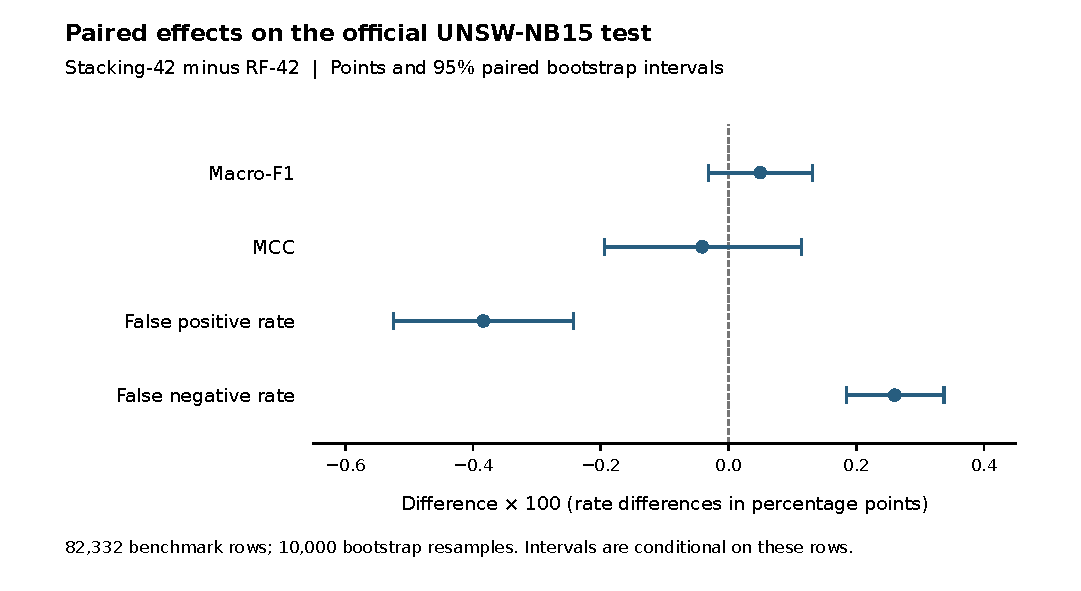
\includegraphics[width=0.95\textwidth]{../results/figures/p16_paired_effects_2026_10_16/paired_effects.pdf}
\caption{Hiệu số Stacking-42 trừ RF-42 và CI 95\% paired bootstrap; trục hoành thể hiện hiệu số nhân 100.}
\label{fig:paired-metrics}
\end{figure}

\section{Chi phí quan sát trong lần chạy lịch sử}
\label{sec:chi-phi}

Bảng~\ref{tab:chi-phi} đối chiếu thời gian huấn luyện, thời gian suy luận trung bình theo lô và dung lượng mô hình ước tính trong lần thực nghiệm ban đầu. Các con số cho thấy Stacking cần nhiều thời gian huấn luyện hơn RF-42 trong lần chạy đó, còn RF-17 có thời gian và kích thước thấp hơn. Chúng mô tả các cấu hình và môi trường lịch sử cụ thể; không phải benchmark lặp lại trên thiết bị triển khai.

\begin{table}[htbp]
\centering
\small
\renewcommand{\arraystretch}{1.3}
\setlength{\tabcolsep}{6pt}
\caption{Chi phí tính toán của ba pipeline trong lần thực nghiệm ban đầu; dung lượng quy đổi sang MiB.}
\label{tab:chi-phi}
\begin{tabularx}{\linewidth}{>{\raggedright\arraybackslash}X S[table-format=2.0] S[table-format=4.3] S[table-format=1.6] S[table-format=3.3]}
\toprule
Pipeline & {\shortstack{Số biến\\gốc}} & {\shortstack{Huấn luyện\\(s)}} & {\shortstack{Suy luận theo lô\\(ms/flow)}} & {\shortstack{Dung lượng\\(MiB)}}\\
\midrule
RF-42 & 42 & 371.244 & 0.008679 & 205.490\\
Stacking-42 & 42 & 980.170 & 0.012445 & 206.216\\
RF-17 & 17 & 57.255 & 0.003562 & 105.044\\
\bottomrule
\end{tabularx}
\end{table}

Trong cùng đợt thực nghiệm, thời gian huấn luyện RF-42 gấp khoảng 6.48 lần RF-17; kích thước ước lượng của RF-17 thấp hơn khoảng 48.88\%. Trường suy luận là thời gian trung bình trên một dòng khi xử lý batch đã đánh giá, không phải độ trễ của một yêu cầu riêng lẻ. Môi trường thư viện gốc chưa được xác định trực tiếp, và kích thước được báo cáo không chứng minh artifact mô hình lịch sử hiện còn tồn tại.

\section{Sai số theo họ tấn công}
\label{sec:attack-family-error}

Phân tích hậu nghiệm theo họ nhãn thật làm rõ khác biệt mà chỉ số tổng thể gộp lại. Trong số 6\,062 mẫu Fuzzers, Stacking-42 bỏ sót 754 mẫu, nhiều hơn RF-42 (621); với Generic, số bỏ sót của Stacking thấp hơn (14 so với 57). Bảng~\ref{tab:attack-family} mở rộng đối chiếu tới đủ chín nhóm Attack và cả ba pipeline. FNR kèm CI Wilson 95\% được trình bày cùng support và số FN để tránh diễn giải đếm lỗi mà không xét quy mô nhóm.

\begin{table}[!htbp]
\centering
\footnotesize
\renewcommand{\arraystretch}{1.15}
\setlength{\tabcolsep}{4pt}
\caption{Số FN, FNR và khoảng tin cậy Wilson 95\% theo từng họ Attack trên official TEST. Mỗi ô mô hình: \textbf{FN / FNR}; dòng dưới là [CI 95\%].}
\label{tab:attack-family}
\begin{tabularx}{\linewidth}{@{}>{\raggedright\arraybackslash}p{3.05cm}r*{3}{>{\centering\arraybackslash}X}@{}}
\toprule
Họ Attack & {$n$} & Stacking-42 & RF-42 & RF-17\\
\midrule
Analysis & 677 & \shortstack[c]{19 / 2.81\%\\{\scriptsize [1.80; 4.34]}} & \shortstack[c]{3 / 0.44\%\\{\scriptsize [0.15; 1.29]}} & \shortstack[c]{1 / 0.15\%\\{\scriptsize [0.03; 0.83]}}\\
Backdoor & 583 & \shortstack[c]{1 / 0.17\%\\{\scriptsize [0.03; 0.97]}} & \shortstack[c]{0 / 0.00\%\\{\scriptsize [0.00; 0.65]}} & \shortstack[c]{0 / 0.00\%\\{\scriptsize [0.00; 0.65]}}\\
DoS & 4089 & \shortstack[c]{9 / 0.22\%\\{\scriptsize [0.12; 0.42]}} & \shortstack[c]{4 / 0.10\%\\{\scriptsize [0.04; 0.25]}} & \shortstack[c]{2 / 0.05\%\\{\scriptsize [0.01; 0.18]}}\\
Exploits & 11132 & \shortstack[c]{49 / 0.44\%\\{\scriptsize [0.33; 0.58]}} & \shortstack[c]{45 / 0.40\%\\{\scriptsize [0.30; 0.54]}} & \shortstack[c]{54 / 0.49\%\\{\scriptsize [0.37; 0.63]}}\\
Fuzzers & 6062 & \shortstack[c]{754 / 12.44\%\\{\scriptsize [11.63; 13.29]}} & \shortstack[c]{621 / 10.24\%\\{\scriptsize [9.51; 11.03]}} & \shortstack[c]{623 / 10.28\%\\{\scriptsize [9.54; 11.07]}}\\
Generic & 18871 & \shortstack[c]{14 / 0.07\%\\{\scriptsize [0.04; 0.12]}} & \shortstack[c]{57 / 0.30\%\\{\scriptsize [0.23; 0.39]}} & \shortstack[c]{3 / 0.02\%\\{\scriptsize [0.01; 0.05]}}\\
Reconnaissance & 3496 & \shortstack[c]{2 / 0.06\%\\{\scriptsize [0.02; 0.21]}} & \shortstack[c]{1 / 0.03\%\\{\scriptsize [0.01; 0.16]}} & \shortstack[c]{19 / 0.54\%\\{\scriptsize [0.35; 0.85]}}\\
Shellcode & 378 & \shortstack[c]{3 / 0.79\%\\{\scriptsize [0.27; 2.31]}} & \shortstack[c]{2 / 0.53\%\\{\scriptsize [0.15; 1.91]}} & \shortstack[c]{6 / 1.59\%\\{\scriptsize [0.73; 3.42]}}\\
Worms & 44 & \shortstack[c]{1 / 2.27\%\\{\scriptsize [0.40; 11.81]}} & \shortstack[c]{1 / 2.27\%\\{\scriptsize [0.40; 11.81]}} & \shortstack[c]{0 / 0.00\%\\{\scriptsize [0.00; 8.03]}}\\
\bottomrule
\end{tabularx}
\end{table}

Các ước lượng này mô tả FN trong từng nhóm nhãn thật trên cùng official TEST, không phải độ chính xác của bộ phân loại đa lớp. Khoảng Wilson là khoảng nhị thức biên theo từng nhóm và pipeline; không phải kiểm định cặp giữa hai mô hình. Những nhóm hiếm, đặc biệt Worms, có khoảng rộng nên tỷ lệ quan sát được cần được đọc thận trọng. Các khác biệt theo nhóm gợi ý vị trí cần khảo sát thêm, nhưng không xác định đặc trưng hay cơ chế nào gây ra lỗi.

\section{Độ nhạy trên novel-vector subset}
\label{sec:novel-vector}

Trong official TEST có 8\,541 dòng mang vector 42 đặc trưng trùng với ít nhất một dòng TRAIN; 73\,791 dòng còn lại tạo thành novel-vector subset. Bảng~\ref{tab:rev-rq4} so sánh Macro-F1 giữa official TEST và subset này, đồng thời báo cáo trực tiếp độ giảm. Đây là một view con của cùng holdout, không phải tập kiểm thử độc lập. Các giá trị giảm ở cả ba pipeline và thứ hạng theo Macro-F1 không đổi, nhưng phép lọc exact-vector không kiểm tra độc lập theo thời gian, host hoặc session. Vì vậy, nó cung cấp một phân tích độ nhạy hữu ích trong benchmark hiện có chứ chưa trả lời đầy đủ khả năng khái quát ngoài split chính thức.
